\documentclass[11pt, a4paper]{article}

\usepackage[czech, slovak]{babel}
\usepackage[utf8]{inputenc}
\usepackage[T1]{fontenc}
\usepackage[unicode]{hyperref}
\usepackage[left=2cm, top=3cm, text={17cm, 24cm}]{geometry}
\usepackage{times}
\usepackage{graphicx}
\usepackage{pdflscape}
\usepackage{hyperref}

\begin{document}
	\begin{titlepage}
		\begin{center}
			
\includegraphics[width=0.77 \linewidth]{FIT_logo.pdf} \\

			\vspace{\stretch{0.382}}

			\Huge{Projekt 1.~časť} \\
			\Huge{Dátový model (ERD), model prípadov užitia} \\
			\LARGE{\textbf{Zoologická záhrada}} \\
			\Large{Databázové systémy}

			\vspace{\stretch{0.618}}
		\end{center}

		{\Large
			\today
			\hfill
			\begin{tabular}{ll}
			Samuel Dobroň & \href{mailto:xdobro23@stud.fit.vutbr.cz}{\texttt{xdobro23@stud.fit.vutbr.cz}} \\
            Juraj Remeň & \href{mailto:xremen02@stud.fit.vutbr.cz}{\texttt{xremen02@stud.fit.vutbr.cz}}
\end{tabular}
}
	\end{titlepage}
		\tableofcontents
		\vspace{21em}
		\section{Zadanie}
		Navrhněte informační systém pro zoologickou zahradu. V zoologické zahradě jsou živočichové umístěni do klecí, výběhů, či do klecí v pavilonech. Živočichové jsou děleni podle třídy, řádu, čeledě, rodu a druhu (např. lama alpaka je v třídě savců, řádu sudokopytníků, v čeledi velbloudovitých, v rodu lama a druhu alpaka). Pro zjednodušení předpokládejte striktně hierarchické dělení živočichů a to, že každý živočich je příslušníkem právě jednoho druhu. Jeden druh živočicha může být v několika výbězích či klecích, a naopak, v jednom výběhu či kleci může být více různých druhů. Systém musí být schopný vyhledávat živočichy podle jejich příslušností do jednotlivých kategorií. Pro každého živočicha je třeba uchovávat informace o datu narození (a případně úmrtí), jméno, historii výsledků měření (hmotnosti, rozměrů, ...), apod.
		\section{Use Case Diagram}
		\scalebox{0.8}{
		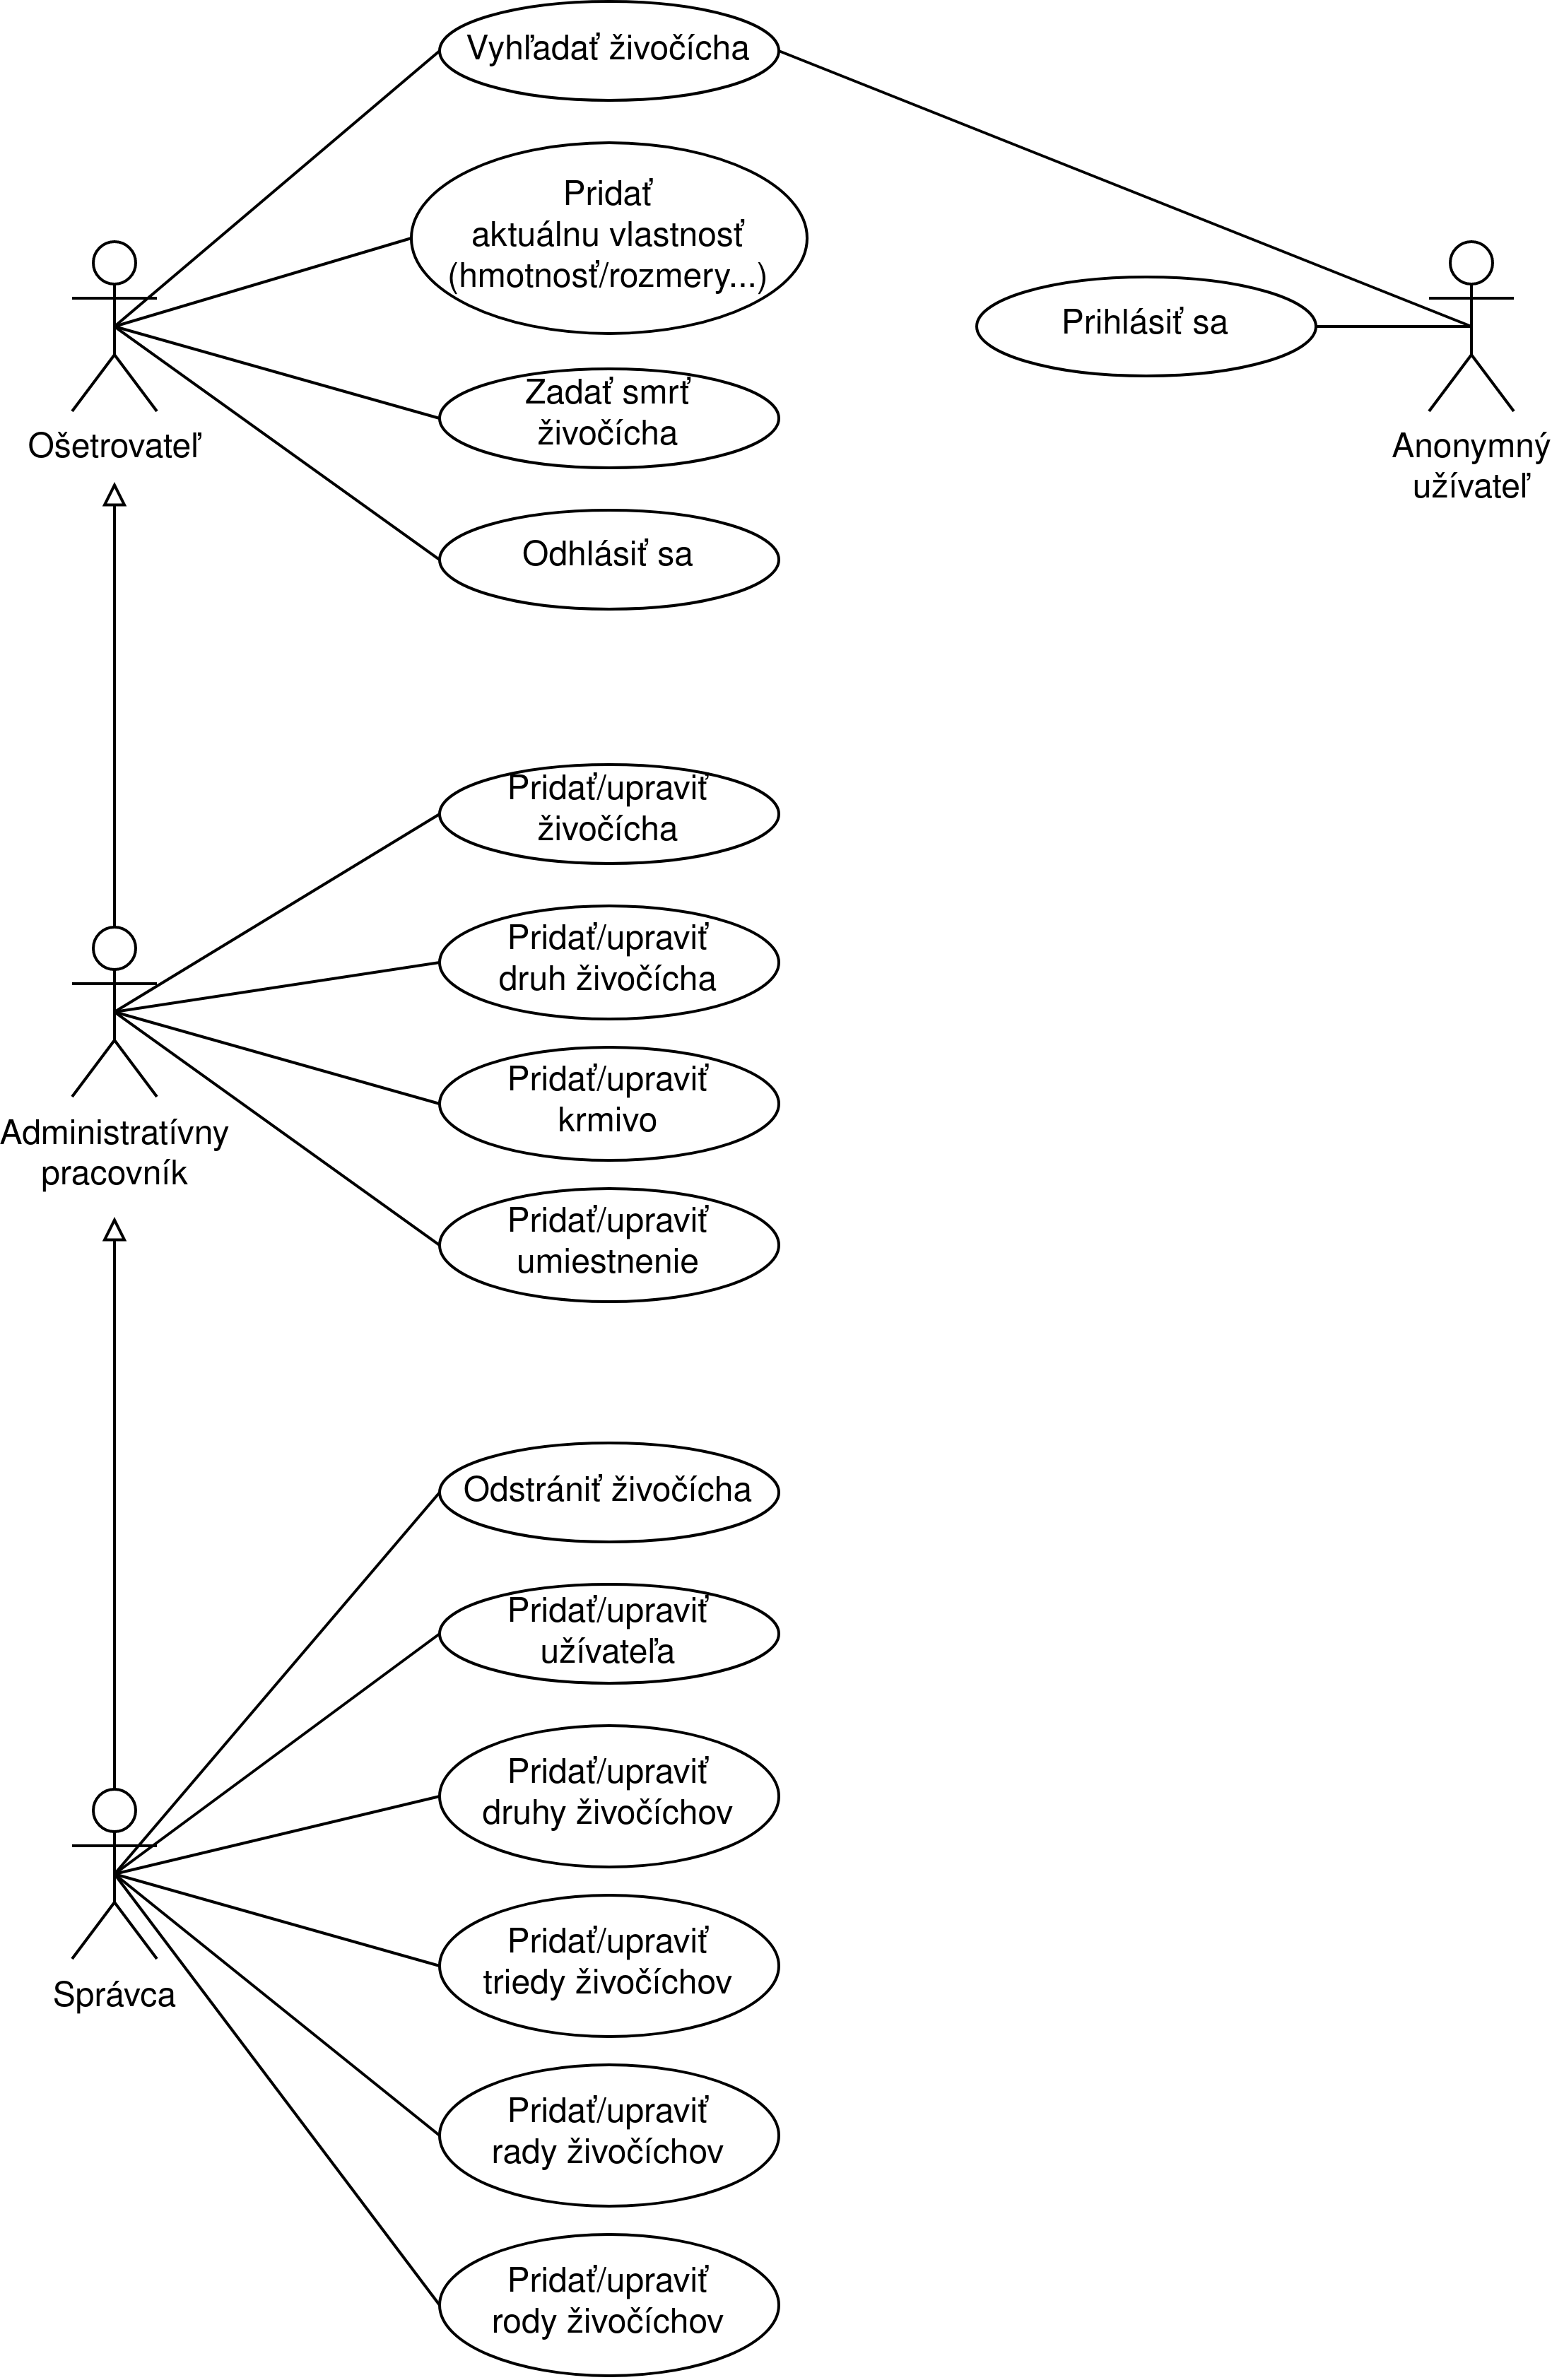
\includegraphics[width=1 \linewidth]{use case.png}}
		\newpage
		\subsection{Popis}
		\label{usecase}
			Diagram prípadov užitia zobrazuje 4 aktérov, ktorí môžu využívať informačný systém.

			\textbf{Anonymný užívateľ} si môže len vyhľadať žívočícha, ide o bežného návštevníka ZOO, prípadne potencionálneho návštevníka, ktorého zaujíma, žo môže v ZOO vidieť. Môže íst samozrejme aj o zamestnanca ZOO, pred prihlásením.

			\textbf{Ošetrovateľ} má priamu zodpovednosť za živočícha, môže si ho teda vyhladať, zadať vlastnosť akou je napríklad \textit{hmostnosť, rozmery, farba, \dots}. Záleží akú vlastnosť je dôležité evidovať pri konkretnom druhu zvieraťa.

			\textbf{Administratívny pracovník} sa priamo o zviera nestará, no je zodpovedný za administratívu okolo zvierat. Dedí teda všetky aspekty aktéra \textbf{Ošetrovateľ} a naviac má svoje vlastné - pridať/upraviť živočícha, či jeho druh, krmivo alebo umiestnenie.

			\textbf{Správca} je správca informačného systému ZOO. Nepredpokladáme žiadne jeho nekalé úmysly a dedí teda aspekty \textbf{Administratívneho pracovníka} a naviac pridáva svoje vlastné. Najmä také, ktoré by \textbf{Ošetrovateľ} či \textbf{Adminsitratívny pracovník} nemal mať k dispozícii. Napríklad odstránenie živočícha, kedže každeho živočícha je potrebné evidovať aj po jeho smrti, nemal by sa nikdy vymazať, no v prípade chyby pri pridávaní nového živočícha, to je žiadúce.

	    \section{Entity Relationship Diagram}
		\scalebox{1.15}{
		\includegraphics[width=0.85 \linewidth]{ER.png}}
		\newpage
		\subsection{Popis}
			ER diagram pozostáva z niekoľkých entít - \textbf{Živočích}, jeho \textbf{Vlastnosti}, \textbf{Umiestnenia} a \textbf{Zamestnanec}, ktorý môže byť jeho ošetrovateľom, prípadne zamestnancom v roli správcu alebo administratívneho pracovníka (viď \hyperref[usecase]{diagram prípadov užitia}).

			\textbf{Zamestnanec} s patričným opravnením, môže meniť umiestnenie \textbf{Živočícha}, na čo slúži entita \textbf{Umiestnenie}. Pre uchovavanie obdobia umiestnenia živočícha sa využívajú atribúty vzťahu -- \textit{od} a \textit{do}.

			Jednou z požiadaviek bola možnosť zaznamenávať rôzne vlastnosti zvieraťa, napríklad váhu, farbu očí a iné. Na tento účel slúži entita \textbf{Vlastnosť}. Typ vlastnosti je špecifikovaný číselníkom \textbf{Typ vlastnosti}.

			Taktiež je potreba uchovávať aj \textbf{triedu}, \textbf{druh}, \textbf{rad}, \textbf{čelaď} a \textbf{rod} živočícha. Kedže sa ale zvierata v ZOO bežne neumiestňujú po 1 kuse, sú tieto typy vlastností uchovávané v číselniku \textbf{Typ živočícha} aby sa predišlo duplicite.
\end{document}